\begin{frame}

  \begin{columns}
    \column{.5\linewidth}
    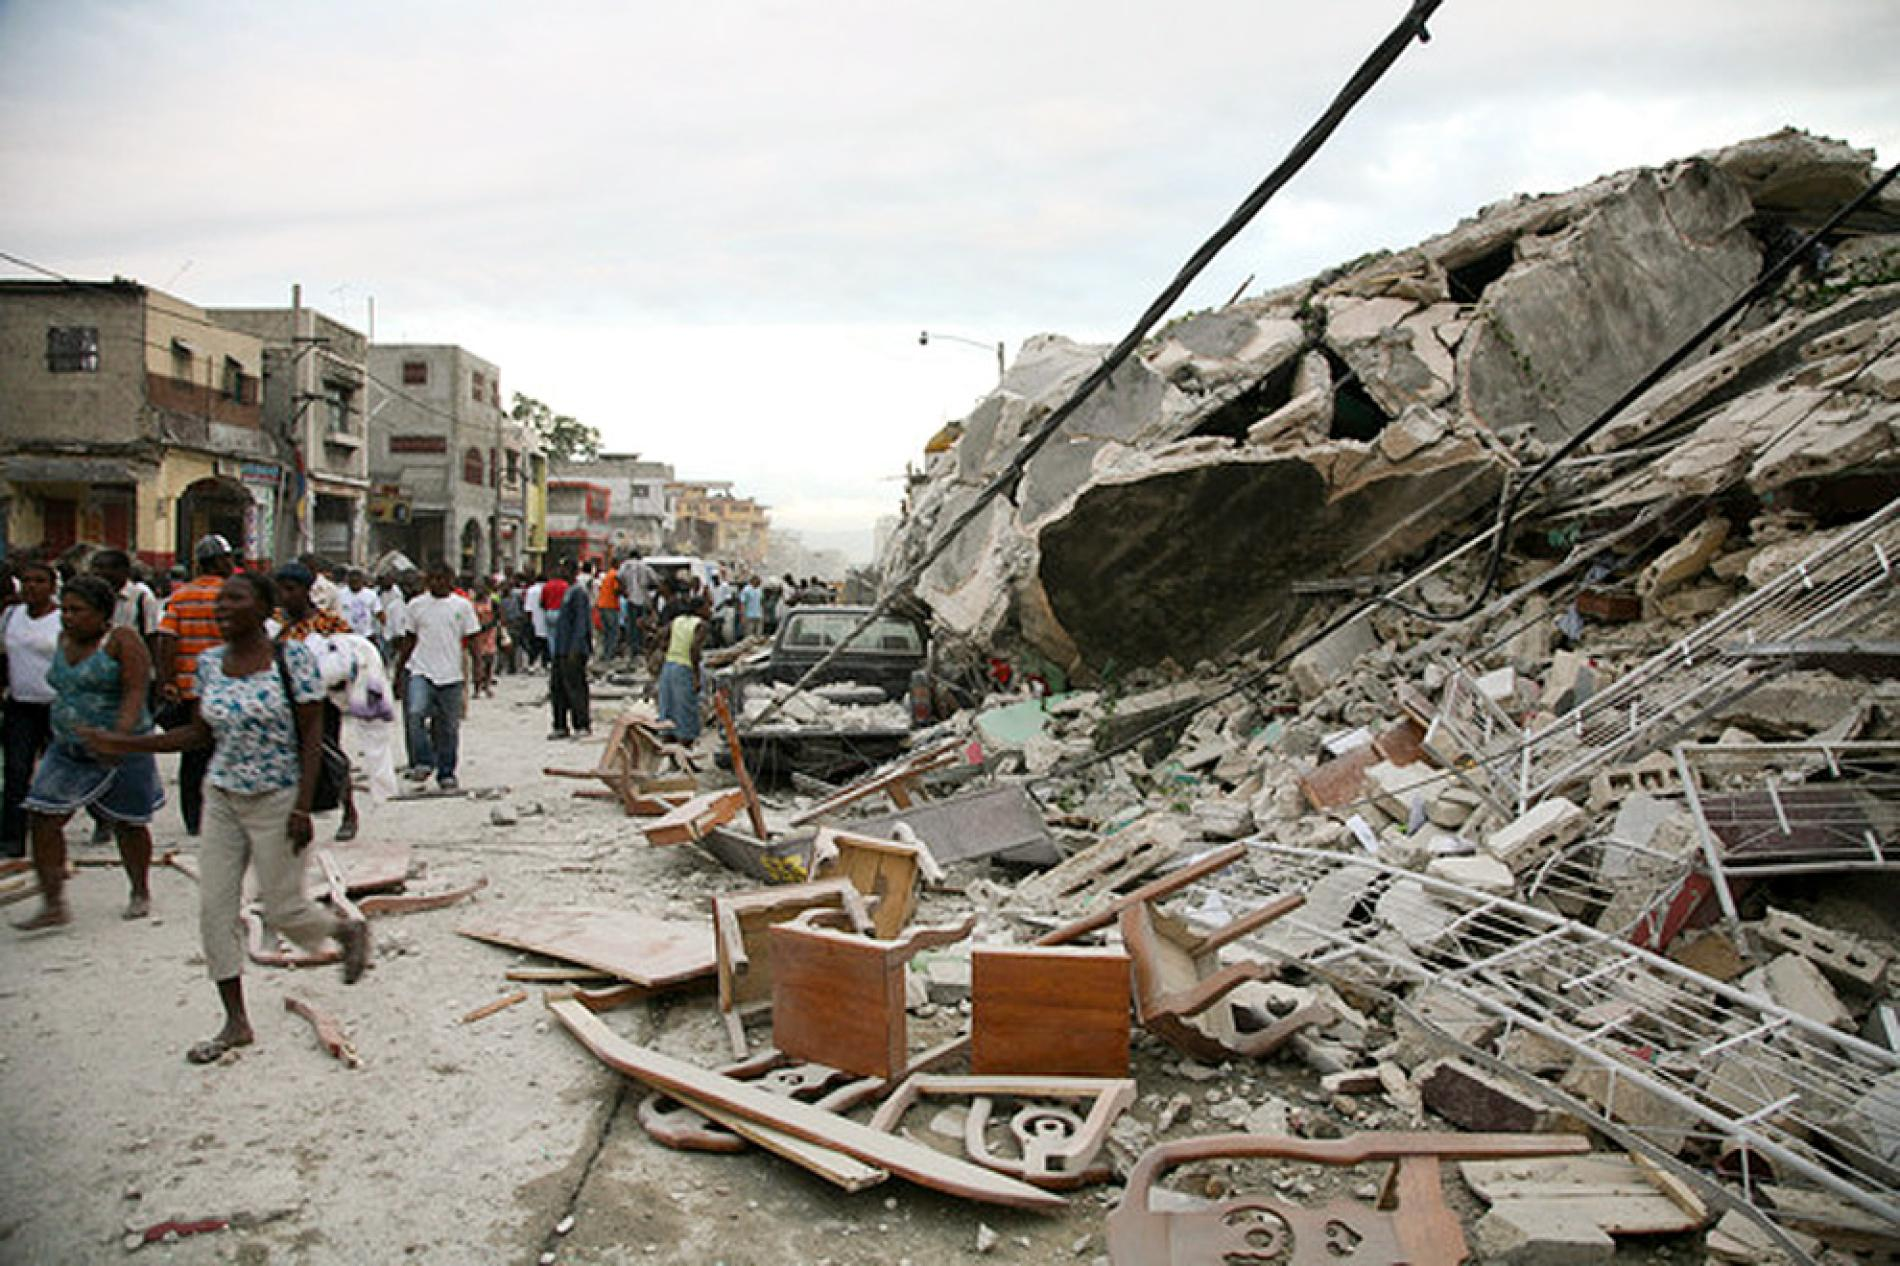
\includegraphics[width=1.0\linewidth]{topic_models/mtanchor/haiti}
    \tiny (Source: National Geographic)

  
  \column{.5\linewidth}
\begin{itemize}
\item Large text collections often require topic triage quickly in low-resource settings (e.g. natural disaster, political instability). 
\item Analysts need to examine multilingual text collections, but are scarce in one or more languages.
\end{itemize}
\end{columns}
\end{frame}


\begin{frame}
  \frametitle{Generative Approaches}
\begin{itemize}
\item Polylingual Topic Model~\cite{mimno-2009}
\item Joint\abr{lda}~\cite{jagarlamudi-2010}
\item Polylingual Tree-based Topic model~\cite{hu-2014-ptlda} 
\item \abr{mcta}~\cite{shi-2016} \pause
\vspace{1cm}
\end{itemize}
\textbf{These methods are slow, assume extensive knowledge about languages, and preclude human refinement.}
\end{frame}



\begin{frame}

\begin{center}
\begin{overprint}
\onslide<1>\centerline{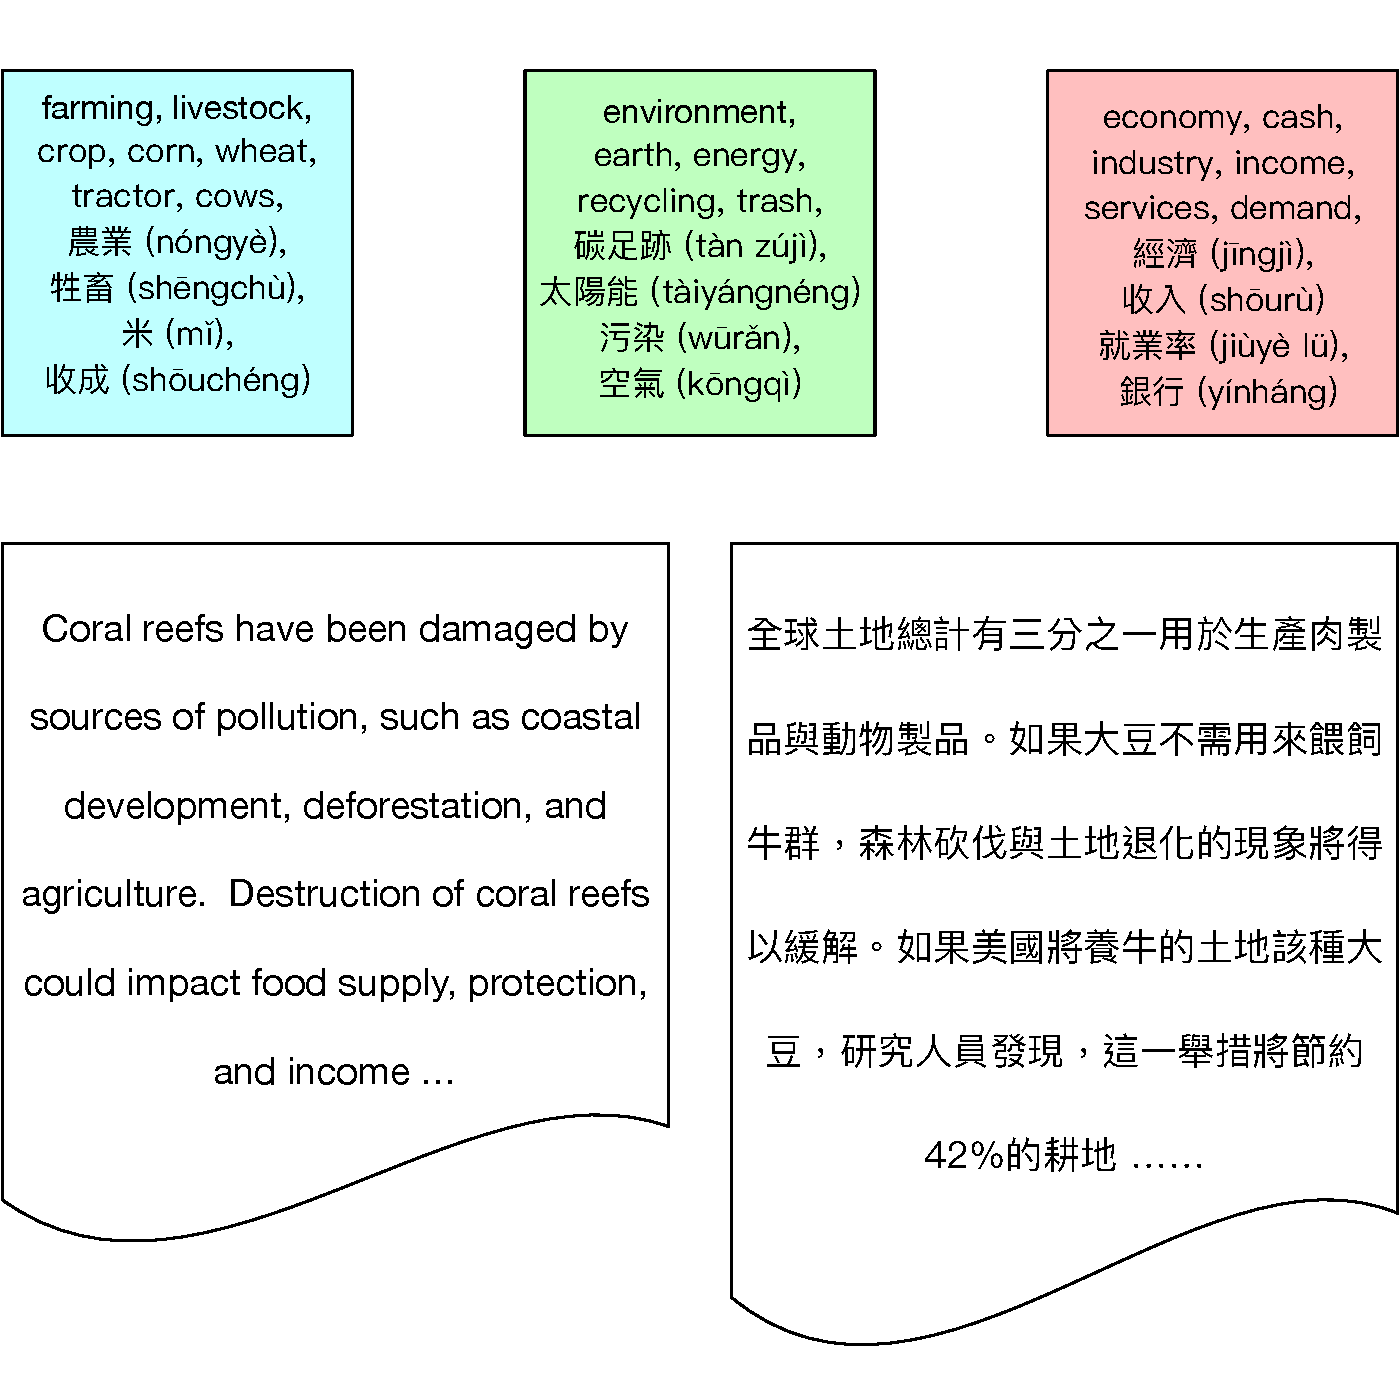
\includegraphics[width=0.5\textwidth]{topic_models/mtanchor/articles1}}
\onslide<2>\centerline{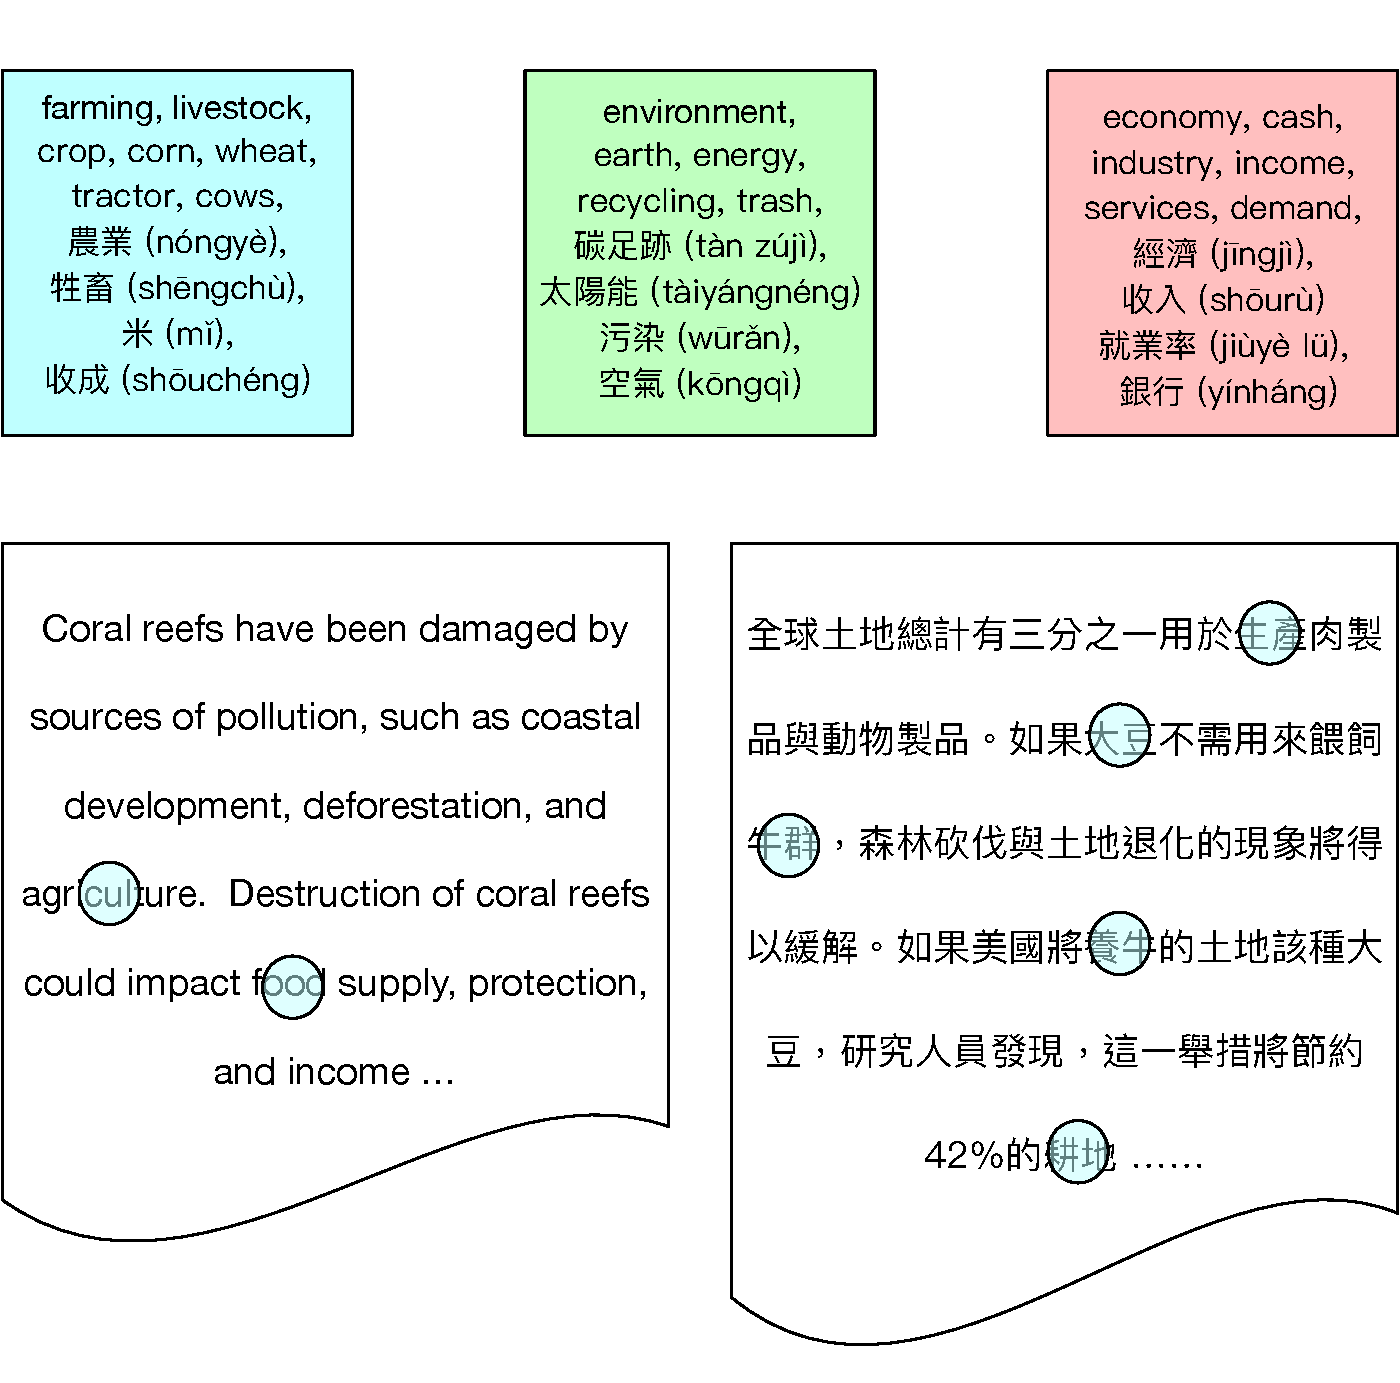
\includegraphics[width=0.5\textwidth]{topic_models/mtanchor/articles2}}
\onslide<3>\centerline{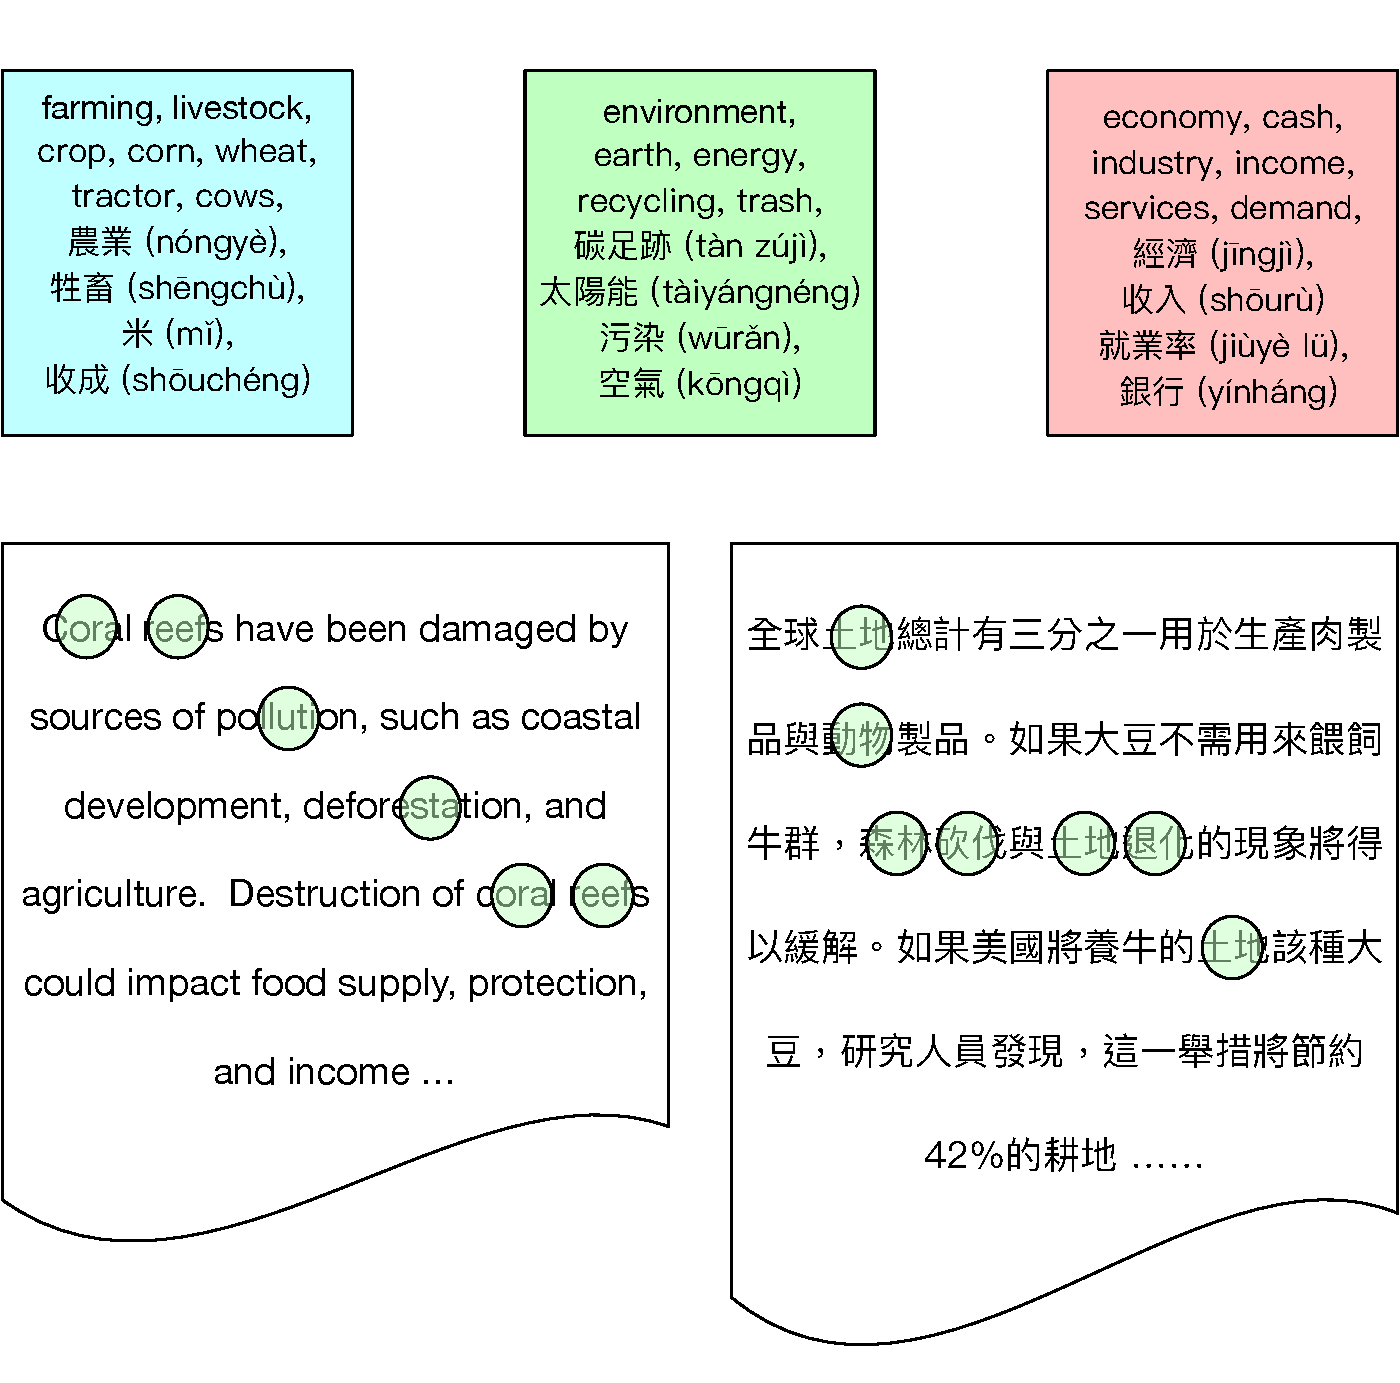
\includegraphics[width=0.5\textwidth]{topic_models/mtanchor/articles3}}
\onslide<4>\centerline{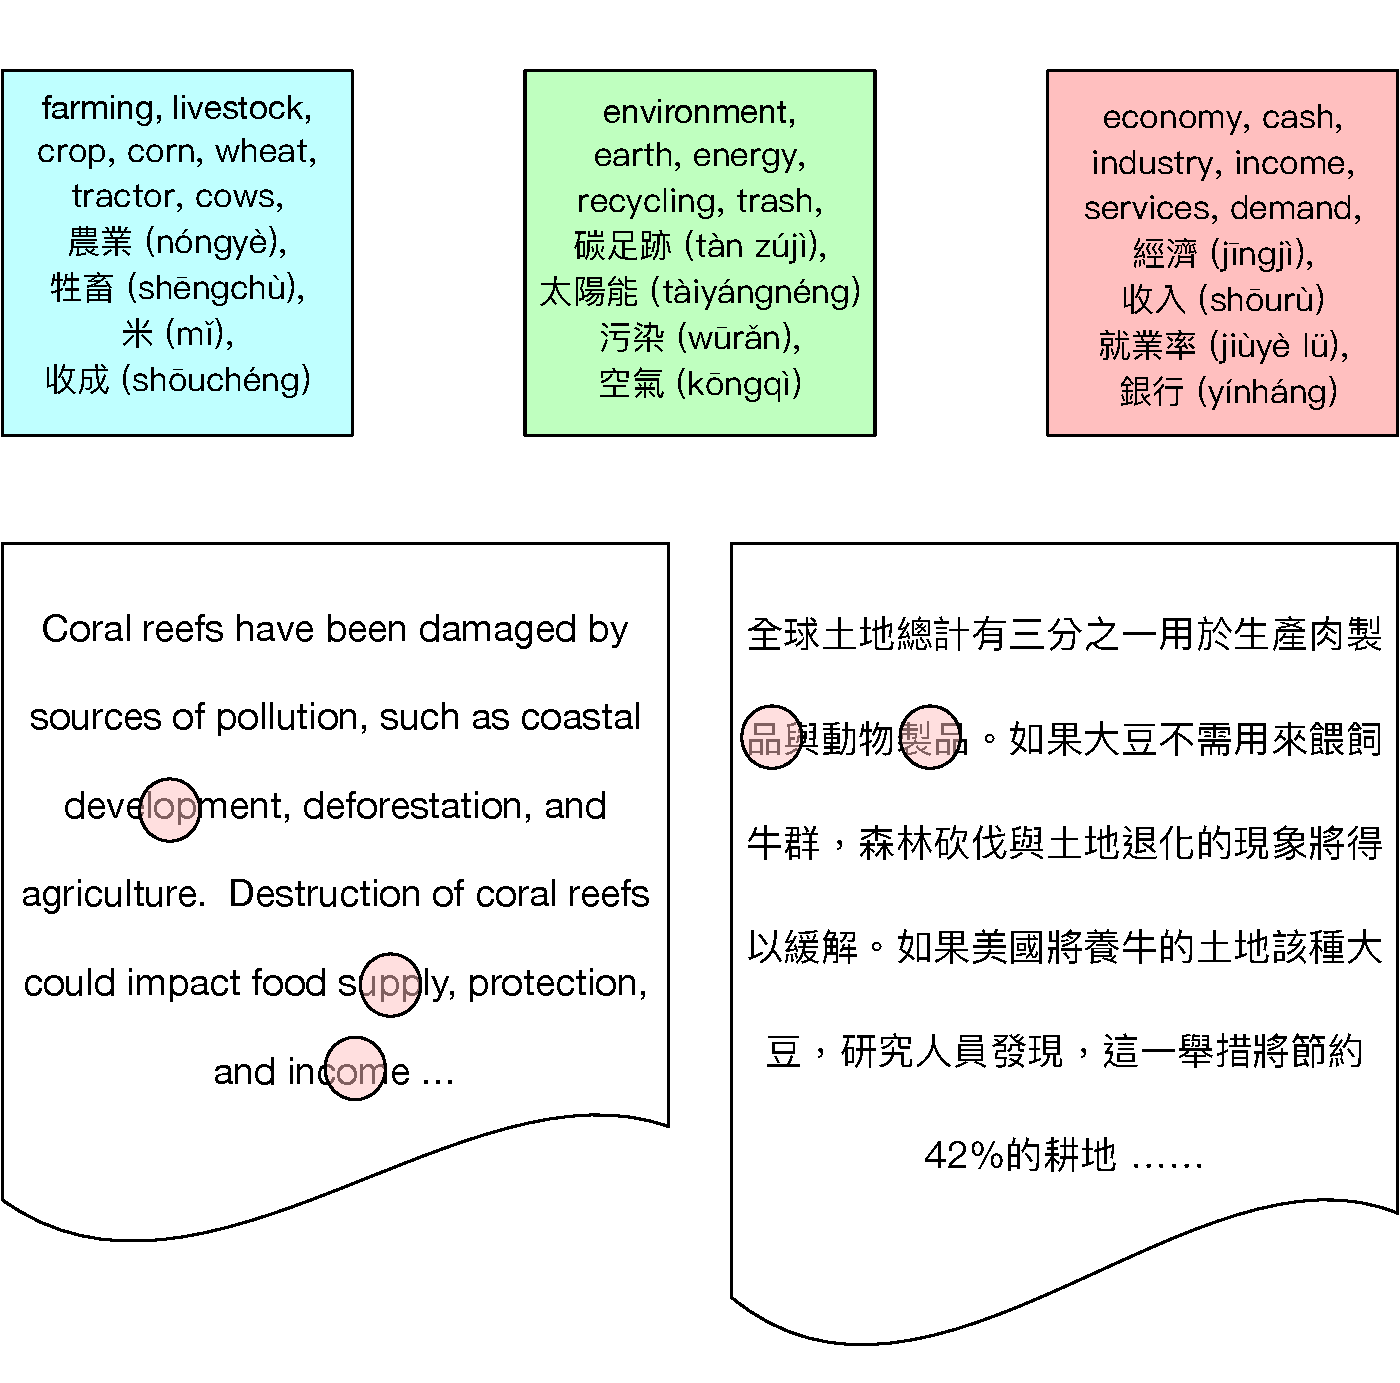
\includegraphics[width=0.5\textwidth]{topic_models/mtanchor/articles4}}
\onslide<5->\centerline{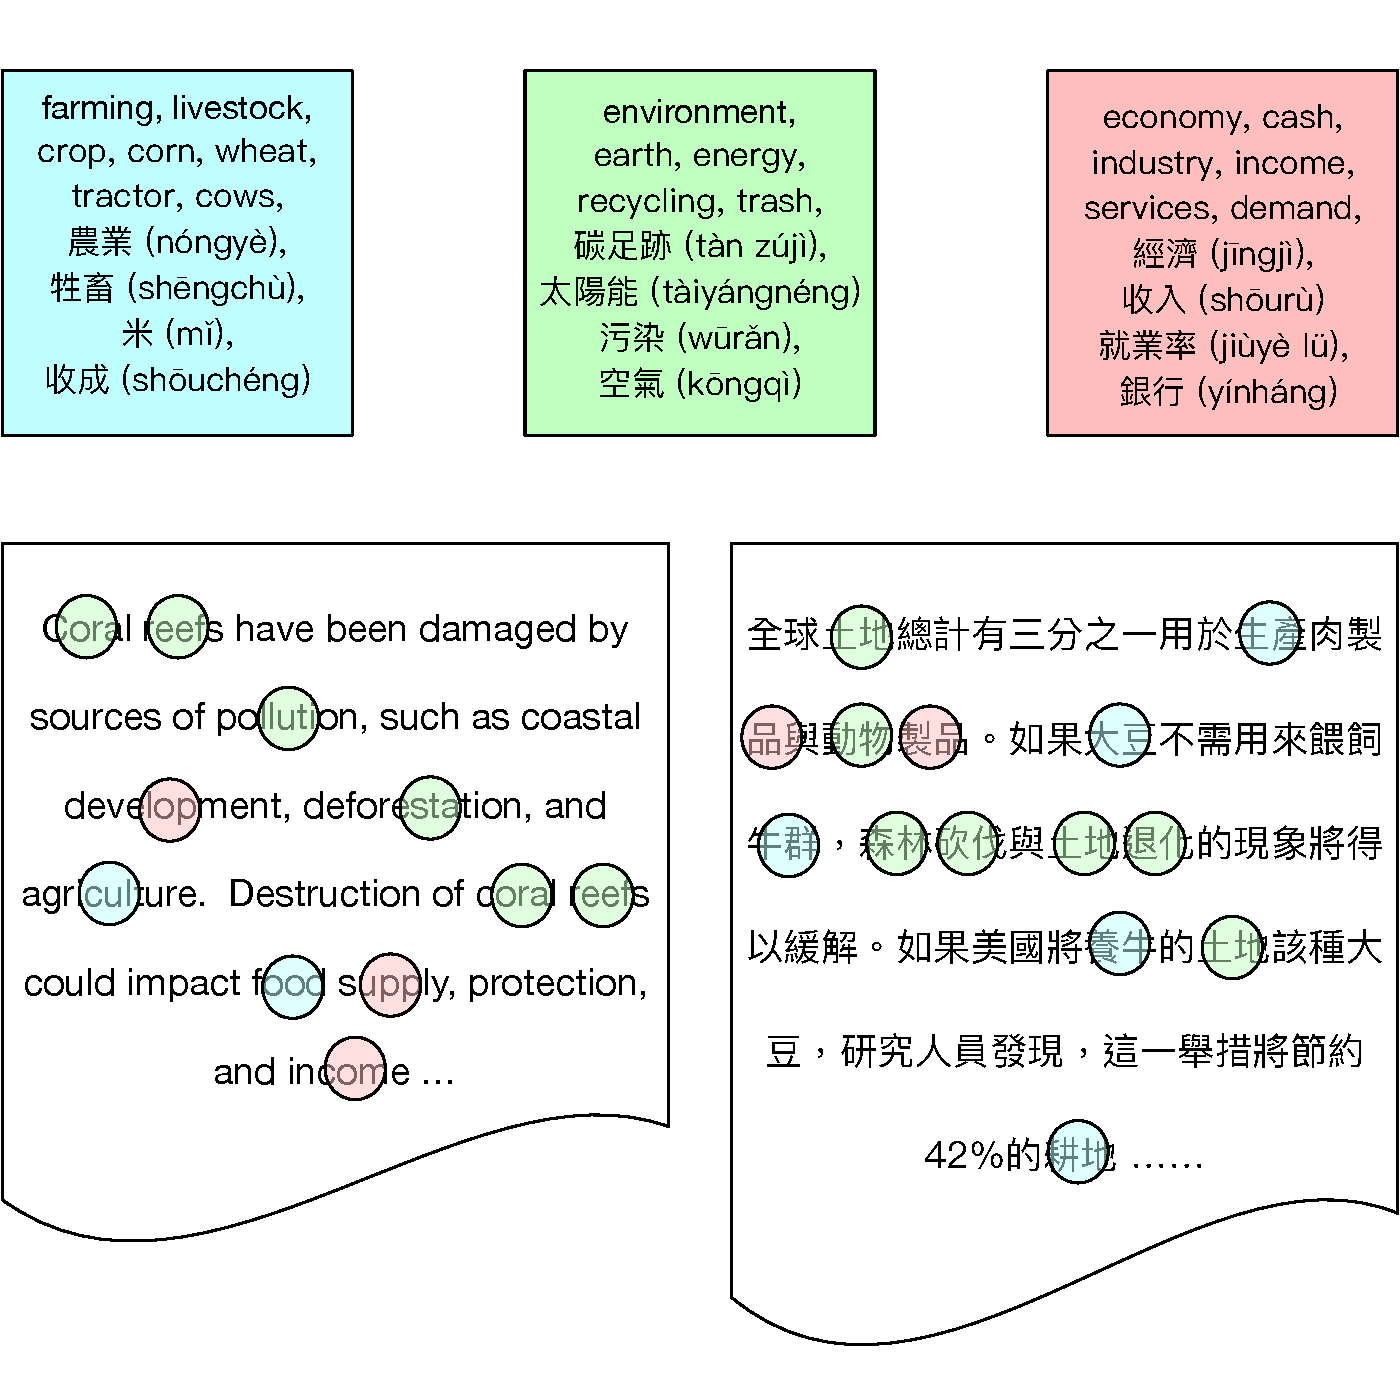
\includegraphics[width=0.5\textwidth]{topic_models/mtanchor/articles5}}
\end{overprint}
\end{center}

\end{frame}



